% Pacotes e configurações padrão do estilo "article"\
% -------------------------------------
\documentclass[a4paper,11pt]{article}
% Layout
% --------------------------------------------------------------------------------
%     Gráficos e layout ----------------------------------------------------------------------

\ifx\pdfmatch\undefined
\else
    \usepackage[T1]{fontenc}
    \usepackage[utf8]{inputenc}
\fi
% xetex:
\ifx\XeTeXinterchartoks\undefined
\else
    \usepackage{fontspec}
    \defaultfontfeatures{Ligatures=TeX}
\fi
% luatex:
\ifx\directlua\undefined
\else
    \usepackage{fontspec}
\fi
% End engine-specific settings

%      Fonte --------------------------------------------------------------------------------
%\usepackage{lmodern}
\usepackage{times}
%     Pacotes adicionados -------------------------------------------------------------------
\usepackage{ae}
%     Língua e hifenização ------------------------------------------------------------------
\usepackage[portuguese]{babel}
\usepackage{hyphenat}
%      Outros --------------------------------------------------------------------------------
\usepackage{hyperref} % Permite Links personalisados usando hyperref
\usepackage{fancyhdr}
\usepackage{sectsty}
\usepackage{float}   % Gerencia melhor o posicionamento das figuras e tabelas
%\usepackage{graphicx}
\usepackage[pdftex]{color,graphicx}
\usepackage{hyperref}
\usepackage{enumerate} % Permite alterar Layout do enumerate
%\usepackage{pdflscape}  % Permite alterar a orientação da pagina para Paisagem
%\usepackage{ifthen}  % Permite usar condicionais ifelse
%\usepackage[table]{xcolor} % Permite alterar as cores das células de uma tabela
\usepackage{amsmath,amssymb} % Ambiente para uso de elementos matemáticos
\usepackage{caption}
\usepackage{subcaption} % permite o uso de multiplas figuras com legenda (ambiente subfigure)
\usepackage{minted} % Ambiente minted para colorir código de programas
\usepackage{natbib} % Para referencia bibliográfica
\usepackage{url}    % Referência de links na internet
%\usepackage{listings} % pacote para apresentar código de programação
\usepackage{indentfirst}  % Para indentar o primeiro parágrafo de cada seção
\usepackage{titling}  % Permite Montar uma página de titulo própria
\usepackage{comment}
% Layout do documento ------------------------------------------------------------------------
%     Bordas e tamanho da página ------------------------------------------------------------
\usepackage{geometry} 
 \geometry{ % Padrõa ABNT para relatórios
 a4paper,
 left=30mm,
 right=20mm,
 top=30mm,
 bottom=20mm
 }
%     Cabeçalho e Rodapé ---------------------------------------------------------------
\pagestyle{fancy}
  \lhead{}
  \chead{}
  \rhead{}
  \lfoot{}
  \cfoot{}
  \rfoot{\thepage}
%     Númeração ------------------------------------------------------------------------

%  \pagenumbering{arabic}
%     Retas do cabeçalho e rodapé ------------------------------------------------------
  \renewcommand{\headrulewidth}{0.5pt}
  \renewcommand{\footrulewidth}{0.5pt}
%     Tamanho da letra de seções e derivadas --------------------------------------------
%  \sectionfont{\normalsize}
%  \subsectionfont{\small}
%     Hiperlinks ------------------------------------------------------------------------
  \hypersetup{
                  colorlinks,
                  citecolor=black,
                  filecolor=black,
                  linkcolor=black,
                  urlcolor=black
                  }
%     Definições do pdf ----------------------------------------------------------------------
\hypersetup{
    unicode=false,          % non-Latin characters in Acrobat’s bookmarks
    pdftoolbar=true,        % show Acrobat’s toolbar?
    pdfmenubar=true,        % show Acrobat’s menu?
    pdffitwindow=false,     % window fit to page when opened
    pdfstartview={FitH},    % fits the width of the page to the window    
    pdfauthor={Rafael Lima},     % author
    pdfnewwindow=true      % links in new window
}
%     Outros ----------------------------------------------------------------------------
      %\renewcommand{\thesection}{(\alph{section})} % muda o estilo de númeração das sections
      % alterando a formatação dos numeradores de lista de itens
      \renewcommand\theenumi{\arabic{enumi}}
      \renewcommand\labelenumi{(\textit{\theenumi})}
	  \renewcommand\theenumii{\arabic{enumii}}
	  \renewcommand\labelenumii{(\textit{\theenumi.\theenumii})}
      
% ---------------------------------------------------------------------------------------




\title{Laboratório - Controle de nível em dois tanques} % Define o título do Relatório

\author{André Almeida}

% Definições Auxiliares ( Macros próprias )
% -----------------------------------------------------------------
%\input{relat_aux.tex} % Arquivo com minhas macros
% ----------------------------------~>ø<~---------------------------------------


\makeatletter
\newcommand{\mathleft}{\@fleqntrue\@mathmargin0pt}
\newcommand{\mathcenter}{\@fleqnfalse}
\makeatother

\begin{document}
% Capa e Índice ---------------------------------------------------------------
%--------------------------------------------------- Capa --------------------------------------------
%\newpage
\begin{figure}[h!]
\centering

\includegraphics[scale=0.9]{img/simb_unb.png}
\label{fig:unb}
\end{figure}

\begin{center}
{\LARGE Universidade de Brasília}\\
Departamento de Engenharia Elétrica\\
Professor: Henrique Cezar Ferreira\\
Disciplina: Controle Digital\\
\end{center}


\vspace{0.18\textheight}

\begin{center}
    \Huge \textbf{\\\thetitle \\}
\end{center}


\vspace*{\fill} % Completa espaço em branco e empurra o resto para o final da página

% Tabela com os nome das pessoas do grupo

\begin{table}[H]
    \begin{tabular}{ll}
        % Nome      & Matrícula
        André Abreu Rodrigues de Almeida & 12/0007100
    \end{tabular}
\end{table}

\vspace{0.5cm}

\begin{center}
    \textbf{Brasília\\
    \the\year} % Coloca o Ano atual
\end{center}

\thispagestyle{empty} % Retira o cabeçalho e o rodapé da página

% ------------------------------------------------- Índice -------------------------------------------
\newpage
% \tableofcontents
% \newpage
% ----------------------------------------------------------------------------------------------------

 % Capa para UnB
% Conteúdo -------------------------------------------------------------------
\pagenumbering{gobble}


\renewcommand*\contentsname{Sumário}
\tableofcontents
\clearpage

\setcounter{page}{1}
\pagenumbering{arabic}

\section{Fundamentação teórica e Modelagem}

A planta sugerida para o trabalho é uma planta com dois tanques não interativos, \textbf{1} e \textbf{2}, preenchidos com líquidos até os níveis $\overline{H_1}$ e $\overline{H_2}$, respectivamente. Os tanques sofrem variação de altura dos níveis de liquido $h_1$ e $h_2$. Duas válvulas, $R_1$ e $R_2$ controlam o fluxo de saída dos tanques \textbf{1} ($\overline{Q} + q_1$) e \textbf{2} ($\overline{Q} + q_2$), respectivamente. O fluxo de entrada no tanque \textbf{1} é $\overline{Q} + q_i$. O tanque \textbf{2} pode receber uma interferência $q_d$.
O sistema descrito pode ser visualizado no diagrama da figura \ref{fig:model}.

\begin{figure}[H]
    \centering
    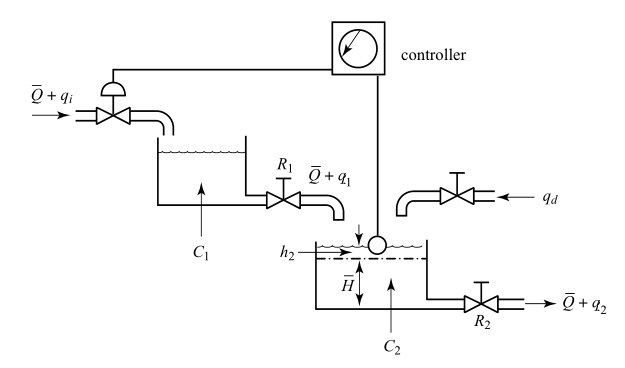
\includegraphics[width=0.8\linewidth]{img/1modelagem/F1-2Tanques.PNG}
    \caption{Modelo - dois tanques com entrada no tanque 1 e perturbação no tanque 2}
    \label{fig:model}
\end{figure}

Este modelo é baseado no capítulo 4 do livro Engenharia de Controle Moderno do autor Katsuhiko Ogata \cite{ogatadinamico}, que descreve sistemas de controle dinâmico similares ao apresentado neste trabalho. A partir desse conceito, com base nas notas de aula e do livro \textit{Discrete-Time Control Systems} \cite{ogatadigital}, também do autor Katsuhiko Ogata, é proposta a discretização e controle pelo método do Lugar das Raízes em tempo discreto.

\subsection{Modelo de um tanque} \label{sect:modmat}

Para modelar o sistema, serão consideradas as leis de Bernoulli simplificadas, como apresentadas no livro do Ogata de controle dinâmico \cite{ogatadinamico}.

\begin{figure}[H]
    \centering
    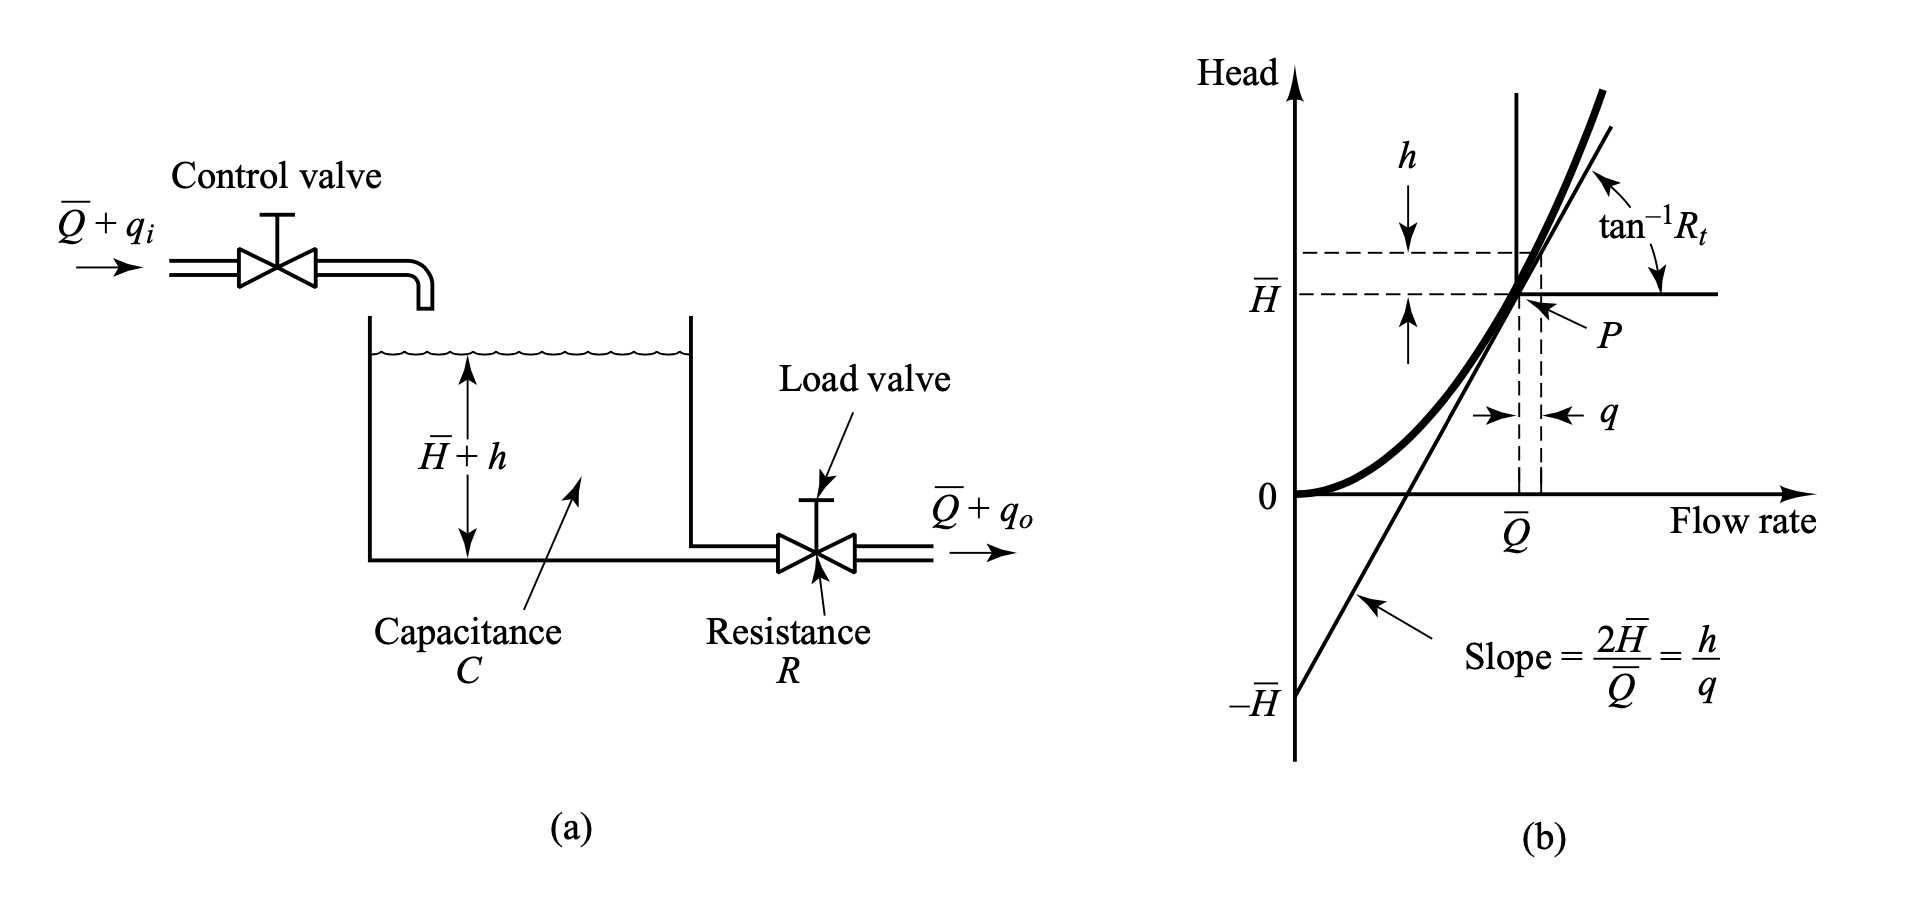
\includegraphics[width=0.8\linewidth]{img/1modelagem/teoria.png}
    \caption{Modelagem de um tanque reservatório de líquido}
    \label{fig:1tq}
\end{figure}

A vazão de um tanque pode ser dada pela equação \ref{eq:vazaoL}, e a resistência pela equação \ref{eq:resistenciaL} no caso de vazão laminar \cite{ogatadinamico}:

\begin{equation}
    Q = K H
    \label{eq:vazaoL}
\end{equation}

\begin{equation}
    R = \frac{dH}{dQ} = \frac{h}{q}
    \label{eq:resistenciaL}
\end{equation}

Já o fluxo turbulento é descrito pelas equações \ref{eq:vazaoT} e \ref{eq:resistenciaT} para vazão e resistência, respectivamente \cite{ogatadinamico}:

\begin{equation}
    Q = K \sqrt{H}
    \label{eq:vazaoT}
\end{equation}

\begin{equation}
    R = \frac{dH}{dQ} = \frac{2h}{q}
    \label{eq:resistenciaT}
\end{equation}

Onde:

\begin{itemize}
    \item $H$ representa o nível do líquido em estado estacionário em $m$
    \item $Q$ representa a vazão em estado estacionário em $m^3/s$
    \item $K$ é um coeficiente em $m^2/s$
    \item $R$ é a resistência à vazão do líquido em $s/m^2$
\end{itemize}

A capacitância de um tanque pode ser obtida pela equação \ref{eq:capacitancia}, que pode ser derivada para a equação diferencial \ref{eq:capdiff} a seguir \cite{ogatadinamico}:

\begin{equation}
    C dh = (q_i - q_o) dt
    \label{eq:capacitancia}
\end{equation}

\begin{equation}
    RC \frac{dh}{dt} + h = R q_i
    \label{eq:capdiff}
\end{equation}

Onde:

\begin{itemize}
    \item $C$ é a capacitância de um tanque em $m^2$
    \item $q_i$ é a pequena variação do fluxo de entrada em $m^3/s$
    \item $q_o$ é a pequena variação do fluxo de saída em $m^3/s$
\end{itemize}

Além disso, adaptando a equação \ref{eq:resistenciaL}, temos que a relação entre a vazão de saída $q_o$ e o nível do tanque é dado pela equação \ref{eq:qohr}.
    
    \begin{equation}
        q_o = \frac{h}{R}
        \label{eq:qohr}
    \end{equation}
    
    Estas equações linearizadas são válidas para pequenas variações em fluxo e nível em relação ao estado estacionário, como é representado na figura \ref{fig:1tq}. Transformando a equação \ref{eq:capdiff} para o domínio de Laplace, obtemos o sistema de primeira ordem mostrado na equação \ref{eq:1tqlaplac}.
    
    \begin{equation}
        \frac{H(s)}{Q_i(s)} = \frac{R}{RCs+1}
        \label{eq:1tqlaplac}
    \end{equation}

Onde:

\begin{itemize}
    \item $H(s) = \mathcal{L}\{h\}$
    \item $Q_i(s) = \mathcal{L}\{q_i\}$
\end{itemize}

E é possível obter a função de transferência do fluxo de saída $Q_o(s)$ em relação à entrada $Q_i(s)$ (equação \ref{eq:qoqilaplac}) utilizando-se a equação \ref{eq:qohr}.

    \begin{equation}
        \frac{Q_o(s)}{Q_i(s)} = \frac{1}{RCs+1}
        \label{eq:qoqilaplac}
    \end{equation}

\subsection{Modelo de dois tanques}

    
    
    Considerando que o tanque 1 pode ser representado pela função de transferência da equação \ref{eq:qoqilaplac} e o tanque 2 pode ser representado pela função de transferência da equação \ref{eq:1tqlaplac}, é possível montar um sistema em malha aberta cuja entrada é $Q_i(s)$ e cuja saída seja $H_2(s)$, conforme a equação \ref{eq:ftma2tqs} a seguir.
    
    \begin{equation}
        \frac{H_2(s)}{Q_i(s)} = \frac{R_2}{(R_1C_1s+1)*(R_2C_2s+1)}
        \label{eq:ftma2tqs}
    \end{equation}
    
    Isso torna o sistema em malha aberta $[Tanque 1; Tanque 2]$, um sistema de segunda ordem no domínio de Laplace. Ao discretizar este sistema, um atraso será adicionado, tornando o sistema pelo menos de ordem três no domínio Z.
    
    A malha do sistema será fechada pelos sensores  incluindo o microcontrolador computadorizado, um segurador de ordem zero e a planta em questão, semelhante ao esquemático da figura \ref{fig:mf}.
    
    \begin{figure}[H]
        \centering
        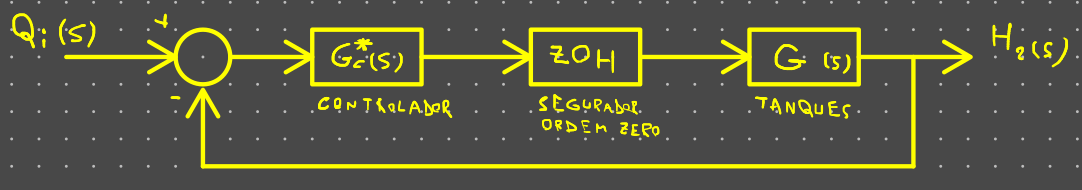
\includegraphics[width=0.6\linewidth]{img/1modelagem/malha-fechada.PNG}
        \caption{Exemplo de diagrama de blocos em malha fechada}
        \label{fig:mf}
    \end{figure}
    
    

\subsection{Capacitância de um tanque}


Galli, Y., em seu trabalho \cite{galli}, interpreta a capacitância como a área da base do tanque. Isto é válido para um tanque cujas paredes são retas e paralelas, como um cubo ou, no caso, um recipiente cuja sessão transversal possui formato de hexágono regular. Dessa forma podemos interpretar a equação \ref{eq:capacitancia} como a equação \ref{eq:capac-area} a seguir:

\begin{equation}
    \frac{dV}{dt} = \frac{d(Ah(t)}{dt} = A \frac{dh(t)}{dt} = q_1(t) - q_o(t) = C \frac{dh(t)}{dt}
    \label{eq:capac-area}
\end{equation}

Portanto, a área e, consequentemente, a capacitância do tanque podem ser calculadas a partir da fórmula apresentada na equação \ref{eq:areahexag}

\begin{equation}
    A = \frac{3 \sqrt{3} * L}{2} = C
    \label{eq:areahexag}
\end{equation}

Onde:

\begin{itemize}
    \item L representa o comprimento do lado do hexágono regular
\end{itemize}

Sabendo que o lado de cada recipiente mede $6cm$, como pode ser visto na figura \ref{fig:ladorecip}, o valor da capacitância do recipiente é $0.00935 m^2$, como apresentado na equação \ref{eq:capacvalue}.

    \begin{figure}[H]
        \centering
        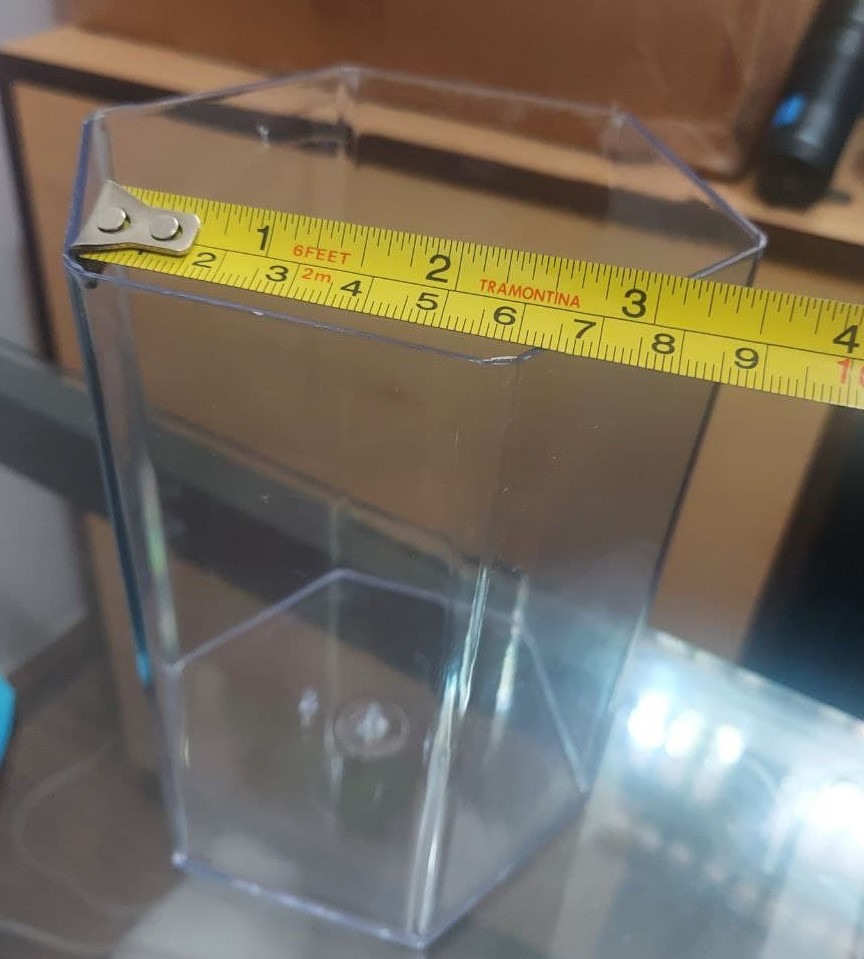
\includegraphics[width=0.5\linewidth]{img/1modelagem/lado-recipiente.jpg}
        \caption{Medição do comprimento do lado do recipiente}
        \label{fig:ladorecip}
    \end{figure}

\begin{equation*}
    C_1 = C_2 = A = \frac{3 \sqrt{3} * 0.06}{2}
\end{equation*}
\begin{equation}
    C_1 = C_2 = 0.00935 m^2
    \label{eq:capacvalue}
\end{equation}


\subsection{Sensores e Atuadores}

Para atuar o sistema, foram escolhidas duas bombas de imersão de 6V corrente contínua que podem ser controladas por um arduino atravéz da utilização de uma ponte H. Dessa maneira será possível alterar a velocidade dos motores para prover água na entrada do tanque 1. Em outras palavras, a partir do controle da tensão na entrada nos motores, a vazão $\overline{Q} + q_i$ pode ser controlada.

Para converter o valor de tensão em vazão, um teste empírico será realizado utilizando sensores de vazão. Com eles será possível traçar uma curva Tensão x Vazão para a variável de controle e assim, será possível controlar a planta através de uma referência de vazão diretamente.

%sensor ultrassônico
%sensor de vazão para calcular R




\subsection{Simulação}

Para entender o funcionamento do sistema aproximado ao real, um modelo no \textit{Simulink} foi criado. Os blocos representando o sistema podem ser vistos nas figuras \ref{fig:simul1} e \ref{fig:simul2}.



\subsection{Escolha do ponto de atuação}

\subsection{Linearização}




% ---------------------------------------------------------------------------------------

\bibliographystyle{abbrv}
\bibliography{references}

% Referências
% Acrescentadas no arquivo references.bib
% para usa-las no texto batsa usar \citep{} ou acrescentar diretamente usando \nocite{}

%\nocite{ogatadinamico}
%\nocite{ogatadigital}
%\nocite{microsoftoutro2}
%\nocite{microsoftoutro3}
%\nocite{microsoftoutro4}


% ---------------------------------------------------------------------------------------
\end{document}
